% Overall architecture of EcoPE-GAT (final model, as-of message passing).
% Compile: pdflatex -output-directory=<dir> figures/src/ecope_gat_architecture.tex
\documentclass[border=4pt]{standalone}
\usepackage{amsmath,amssymb}
\usepackage{tikz}
\usetikzlibrary{arrows.meta,calc,positioning,patterns}
\renewcommand{\familydefault}{\sfdefault}

\definecolor{cBlue}{HTML}{2A5DA8}   \definecolor{fBlue}{HTML}{EEF3FB}
\definecolor{cPurp}{HTML}{6B4FA0}   \definecolor{fPurp}{HTML}{F3EFFA}
\definecolor{cOran}{HTML}{C9861E}   \definecolor{fOran}{HTML}{FDF6E8}
\definecolor{cRed}{HTML}{B5474B}    \definecolor{fRed}{HTML}{FBEDED}
\definecolor{cGreen}{HTML}{3F7F4A}  \definecolor{fGreen}{HTML}{EEF6EF}
\definecolor{cLate}{HTML}{E07B39}

\begin{document}
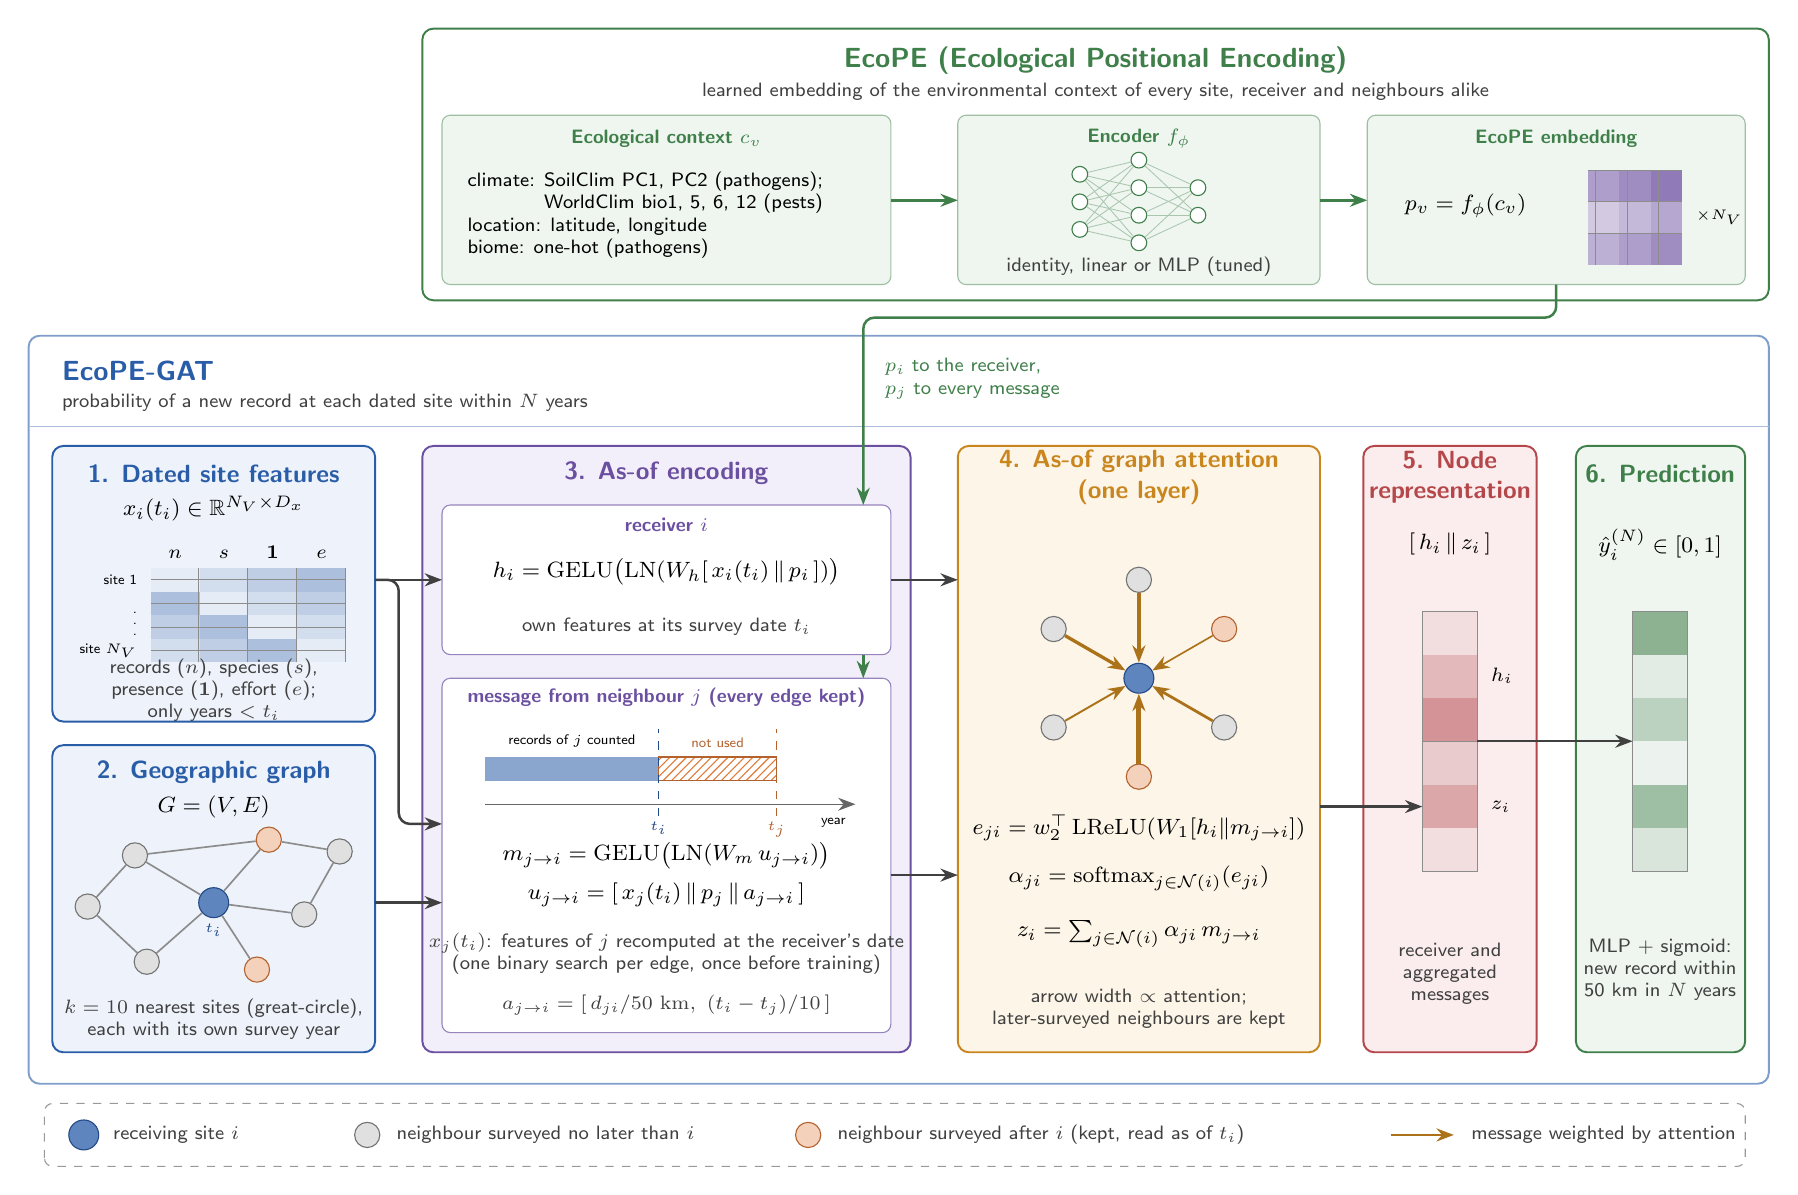
\begin{tikzpicture}[font=\sffamily\small, >={Stealth[length=2.2mm]},
  panel/.style={draw=#1, rounded corners=4pt, line width=0.7pt},
  ptitle/.style={font=\sffamily\bfseries\small, text=#1, align=center},
  note/.style={font=\sffamily\scriptsize, text=black!75, align=center},
  eq/.style={font=\footnotesize},
  site/.style={circle, draw=black!55, fill=black!12, minimum size=3.2mm, inner sep=0pt},
  late/.style={circle, draw=cLate!80!black, fill=cLate!35, minimum size=3.2mm, inner sep=0pt},
  target/.style={circle, draw=cBlue!80!black, fill=cBlue!75, minimum size=3.8mm, inner sep=0pt},
  flow/.style={->, line width=0.9pt, black!75},
  ecoflow/.style={->, line width=0.9pt, cGreen}]

% ================================================================ EcoPE (top)
\draw[panel=cGreen, fill=white] (4.7,9.55) rectangle (21.8,13.0);
\node[ptitle=cGreen, font=\sffamily\bfseries\normalsize] at (13.25,12.6) {EcoPE (Ecological Positional Encoding)};
\node[note] at (13.25,12.2) {learned embedding of the environmental context of every site, receiver and neighbours alike};
% context
\draw[cGreen!50, rounded corners=3pt, fill=fGreen] (4.95,9.75) rectangle (10.65,11.9);
\node[font=\sffamily\scriptsize\bfseries, text=cGreen] at (7.8,11.6) {Ecological context $c_v$};
\node[font=\sffamily\scriptsize, align=left, anchor=north west] at (5.15,11.3)
  {climate: SoilClim PC1, PC2 (pathogens);\\ \phantom{climate: }WorldClim bio1, 5, 6, 12 (pests)\\ location: latitude, longitude\\ biome: one-hot (pathogens)};
% encoder
\draw[cGreen!50, rounded corners=3pt, fill=fGreen] (11.5,9.75) rectangle (16.1,11.9);
\node[font=\sffamily\scriptsize\bfseries, text=cGreen] at (13.8,11.6) {Encoder $f_\phi$};
\foreach \y in {0,1,2} \node[circle, draw=cGreen, fill=white, minimum size=2mm, inner sep=0] (a\y) at (13.05,10.45+0.35*\y) {};
\foreach \y in {0,1,2,3} \node[circle, draw=cGreen, fill=white, minimum size=2mm, inner sep=0] (b\y) at (13.8,10.28+0.35*\y) {};
\foreach \y in {0,1} \node[circle, draw=cGreen, fill=white, minimum size=2mm, inner sep=0] (o\y) at (14.55,10.63+0.35*\y) {};
\foreach \i in {0,1,2} \foreach \j in {0,1,2,3} \draw[cGreen!45, line width=0.3pt] (a\i) -- (b\j);
\foreach \i in {0,1,2,3} \foreach \j in {0,1} \draw[cGreen!45, line width=0.3pt] (b\i) -- (o\j);
\node[note] at (13.8,9.98) {identity, linear or MLP (tuned)};
% embedding
\draw[cGreen!50, rounded corners=3pt, fill=fGreen] (16.7,9.75) rectangle (21.5,11.9);
\node[font=\sffamily\scriptsize\bfseries, text=cGreen] at (19.1,11.6) {EcoPE embedding};
\node[eq] at (17.95,10.75) {$p_v = f_\phi(c_v)$};
\foreach \r/\s in {0/55,1/30,2/45} \foreach \c in {0,1,2} {
  \pgfmathsetmacro{\sh}{int(\s+\c*10)}
  \fill[cPurp!\sh] (19.5+0.4*\c,11.2-0.4*\r-0.4) rectangle ++(0.4,0.4);
}
\draw[black!45] (19.5,10.0) grid[step=0.4] (20.7,11.2);
\node[font=\sffamily\tiny, anchor=west] at (20.75,10.6) {$\times N_V$};
\draw[ecoflow] (10.65,10.82) -- (11.5,10.82);
\draw[ecoflow] (16.1,10.82) -- (16.7,10.82);

% ================================================================ main frame
\draw[panel=cBlue!60] (-0.3,-0.4) rectangle (21.8,9.1);
\node[ptitle=cBlue, font=\sffamily\bfseries\normalsize, anchor=west] at (0,8.65) {EcoPE-GAT};
\node[note, anchor=west] at (0,8.25) {probability of a new record at each dated site within $N$ years};
\draw[cBlue!40] (-0.3,7.95) -- (21.8,7.95);

% ---------------------------------------------------------------- 1. dated features
\draw[panel=cBlue, fill=fBlue] (0,4.2) rectangle (4.1,7.7);
\node[ptitle=cBlue] at (2.05,7.35) {1. Dated site features};
\node[eq] at (2.05,6.9) {$x_i(t_i) \in \mathbb{R}^{N_V \times D_x}$};
\foreach \c/\lab in {0/{$n$},1/{$s$},2/{$\mathbf{1}$},3/{$e$}} {
  \node[font=\sffamily\scriptsize, anchor=south] at (1.25+0.62*\c+0.31,6.15) {\lab};
}
\foreach \r in {0,...,3} \foreach \c in {0,...,3} {
  \pgfmathsetmacro{\shade}{int(mod(\r*3+\c*5,4)*9+12)}
  \fill[cBlue!\shade] (1.25+0.62*\c,6.15-0.3*\r-0.3) rectangle ++(0.62,0.3);
}
\draw[black!45] (1.25,4.95) grid[xstep=0.62, ystep=0.3] (3.73,6.15);
\node[font=\sffamily\tiny, anchor=east] at (1.2,6.0) {site 1};
\node[font=\sffamily\tiny, anchor=east] at (1.2,5.55) {$\vdots$};
\node[font=\sffamily\tiny, anchor=east] at (1.2,5.1) {site $N_V$};
\node[note] at (2.05,4.6) {records ($n$), species ($s$),\\ presence ($\mathbf{1}$), effort ($e$);\\ only years $< t_i$};

% ---------------------------------------------------------------- 2. geographic graph
\draw[panel=cBlue, fill=fBlue] (0,0) rectangle (4.1,3.9);
\node[ptitle=cBlue] at (2.05,3.55) {2. Geographic graph};
\node[eq] at (2.05,3.12) {$G = (V, E)$};
\node[target] (g0) at (2.05,1.9) {};
\node[site] (g1) at (1.05,2.5) {};  \node[late] (g2) at (2.75,2.7) {};
\node[site] (g3) at (3.2,1.75) {};  \node[late] (g4) at (2.6,1.05) {};
\node[site] (g5) at (1.2,1.15) {};  \node[site] (g6) at (0.45,1.85) {};
\node[site] (g7) at (3.65,2.55) {};
\foreach \a/\b in {g1/g0,g2/g0,g3/g0,g4/g0,g5/g0,g6/g1,g6/g5,g7/g2,g7/g3,g1/g2}
  \draw[black!45, line width=0.6pt] (\a) -- (\b);
\node[font=\sffamily\tiny, text=cBlue!80!black] at (2.05,1.55) {$t_i$};
\node[note] at (2.05,0.42) {$k = 10$ nearest sites (great-circle),\\ each with its own survey year};

% ---------------------------------------------------------------- 3. as-of encoding
\draw[panel=cPurp, fill=fPurp] (4.7,0) rectangle (10.9,7.7);
\node[ptitle=cPurp] at (7.8,7.35) {3. As-of encoding};
% receiver
\draw[cPurp!70, rounded corners=3pt, fill=white] (4.95,5.05) rectangle (10.65,6.95);
\node[font=\sffamily\scriptsize\bfseries, text=cPurp] at (7.8,6.7) {receiver $i$};
\node[eq] at (7.8,6.1) {$h_i = \mathrm{GELU}\big(\mathrm{LN}(W_h[\,x_i(t_i) \,\|\, p_i\,])\big)$};
\node[note] at (7.8,5.4) {own features at its survey date $t_i$};
% message
\draw[cPurp!70, rounded corners=3pt, fill=white] (4.95,0.25) rectangle (10.65,4.75);
\node[font=\sffamily\scriptsize\bfseries, text=cPurp] at (7.8,4.5) {message from neighbour $j$ (every edge kept)};
\draw[->, black!60] (5.5,3.15) -- (10.2,3.15);
\node[font=\sffamily\tiny, anchor=north east] at (10.2,3.1) {year};
\fill[cBlue!55] (5.5,3.45) rectangle (7.7,3.75);
\fill[pattern=north east lines, pattern color=cLate] (7.7,3.45) rectangle (9.2,3.75);
\draw[cLate!80!black, line width=0.5pt] (7.7,3.45) rectangle (9.2,3.75);
\draw[dashed, cBlue!80!black] (7.7,3.0) -- (7.7,4.1);
\draw[dashed, cLate!80!black] (9.2,3.0) -- (9.2,4.1);
\node[font=\sffamily\tiny, text=cBlue!80!black, anchor=north] at (7.7,3.05) {$t_i$};
\node[font=\sffamily\tiny, text=cLate!80!black, anchor=north] at (9.2,3.05) {$t_j$};
\node[font=\sffamily\tiny, anchor=south] at (6.6,3.75) {records of $j$ counted};
\node[font=\sffamily\tiny, text=cLate!80!black, anchor=south] at (8.45,3.75) {not used};
\node[eq] at (7.8,2.5) {$m_{j\to i} = \mathrm{GELU}\big(\mathrm{LN}(W_m\, u_{j\to i})\big)$};
\node[eq] at (7.8,2.0) {$u_{j\to i} = [\,x_j(t_i) \,\|\, p_j \,\|\, a_{j\to i}\,]$};
\node[note] at (7.8,1.25) {$x_j(t_i)$: features of $j$ recomputed at the receiver's date\\ (one binary search per edge, once before training)};
\node[note] at (7.8,0.6) {$a_{j\to i} = [\,d_{ji}/50\ \mathrm{km},\ (t_i - t_j)/10\,]$};

% ---------------------------------------------------------------- 4. attention
\draw[panel=cOran, fill=fOran] (11.5,0) rectangle (16.1,7.7);
\node[ptitle=cOran] at (13.8,7.3) {4. As-of graph attention\\ (one layer)};
\begin{scope}[shift={(13.8,4.75)}]
  \node[target] (c) at (0,0) {};
  \foreach \ang/\kind/\w in {90/site/1.4, 30/late/0.6, -30/site/1.0, -90/late/1.8, -150/site/0.7, 150/site/1.2} {
    \node[\kind] (n\ang) at (\ang:1.25) {};
    \draw[->, cOran!85!black, line width=\w pt] (n\ang) -- (c);
  }
\end{scope}
\node[eq] at (13.8,2.85) {$e_{ji} = w_2^{\top}\,\mathrm{LReLU}(W_1[h_i \| m_{j\to i}])$};
\node[eq] at (13.8,2.2) {$\alpha_{ji} = \mathrm{softmax}_{j \in \mathcal{N}(i)}(e_{ji})$};
\node[eq] at (13.8,1.5) {$z_i = \textstyle\sum_{j \in \mathcal{N}(i)} \alpha_{ji}\, m_{j\to i}$};
\node[note] at (13.8,0.55) {arrow width $\propto$ attention;\\ later-surveyed neighbours are kept};

% ---------------------------------------------------------------- 5. node representation
\draw[panel=cRed, fill=fRed] (16.65,0) rectangle (18.85,7.7);
\node[ptitle=cRed] at (17.75,7.3) {5. Node\\ representation};
\node[eq] at (17.75,6.45) {$[\,h_i \,\|\, z_i\,]$};
\foreach \r in {0,...,5} {
  \pgfmathsetmacro{\shade}{int(mod(\r*7,5)*10+18)}
  \fill[cRed!\shade] (17.4,5.6-0.55*\r-0.55) rectangle ++(0.7,0.55);
}
\draw[black!45] (17.4,2.3) rectangle (18.1,5.6);
\draw[black!45] (17.4,3.95) -- (18.1,3.95);
\node[font=\sffamily\scriptsize, anchor=west] at (18.15,4.78) {$h_i$};
\node[font=\sffamily\scriptsize, anchor=west] at (18.15,3.12) {$z_i$};
\node[note] at (17.75,1.0) {receiver and\\ aggregated\\ messages};

% ---------------------------------------------------------------- 6. prediction
\draw[panel=cGreen, fill=fGreen] (19.35,0) rectangle (21.5,7.7);
\node[ptitle=cGreen] at (20.42,7.35) {6. Prediction};
\node[eq] at (20.42,6.45) {$\hat{y}_i^{(N)} \in [0,1]$};
\foreach \r/\s in {0/60,1/15,2/35,3/10,4/50,5/20} {
  \fill[cGreen!\s] (20.07,5.6-0.55*\r-0.55) rectangle ++(0.7,0.55);
}
\draw[black!45] (20.07,2.3) rectangle (20.77,5.6);
\node[note] at (20.42,1.05) {MLP + sigmoid:\\ new record within\\ 50 km in $N$ years};

% ---------------------------------------------------------------- arrows
\draw[flow] (4.1,6.0) -- (4.95,6.0);              % features -> receiver
\draw[flow, rounded corners=4pt] (4.1,6.0) -- (4.4,6.0) -- (4.4,2.9) -- (4.95,2.9);  % features -> message (x_j)
\draw[flow] (4.1,1.9) -- (4.95,1.9);              % graph -> message (edges, dates)
\draw[ecoflow, rounded corners=4pt] (19.1,9.75) -- (19.1,9.33) -- (10.3,9.33) -- (10.3,6.95);  % p_i, p_j
\draw[ecoflow] (10.3,5.05) -- (10.3,4.75);
\node[font=\sffamily\scriptsize, text=cGreen, anchor=west, align=left] at (10.45,8.55) {$p_i$ to the receiver,\\ $p_j$ to every message};
\draw[flow] (10.65,6.0) -- (11.5,6.0);            % h_i -> attention
\draw[flow] (10.65,2.25) -- (11.5,2.25);          % m -> attention
\draw[flow] (16.1,3.12) -- (17.4,3.12);           % z_i -> representation
\draw[flow] (18.1,3.95) -- (20.07,3.95);          % -> prediction

% ---------------------------------------------------------------- legend
\begin{scope}[shift={(0.4,-1.05)}]
  \draw[black!40, dashed, rounded corners=3pt] (-0.5,-0.4) rectangle (21.1,0.4);
  \node[target] at (0,0) {};  \node[note, anchor=west] at (0.25,0) {receiving site $i$};
  \node[site] at (3.6,0) {};  \node[note, anchor=west] at (3.85,0) {neighbour surveyed no later than $i$};
  \node[late] at (9.2,0) {};  \node[note, anchor=west] at (9.45,0) {neighbour surveyed after $i$ (kept, read as of $t_i$)};
  \draw[->, cOran!85!black, line width=1pt] (16.6,0) -- (17.4,0);
  \node[note, anchor=west] at (17.5,0) {message weighted by attention};
\end{scope}
\end{tikzpicture}
\end{document}
